
% TODO: not relevant here, move to introduction
%Agricultural technologies have been a source of innovation since the dawn of humanity. The quest for more efficient food
%production has driven significant research, and above all, automation stands out as a paramount achievement in the
%modern world. A great tool to improve the automation process is \gls{IoT}, a concept that refers to the interconnection
%of physical devices in a diffused network; each device collects valuable and localized information that is used to
%improve efficiency, productivity, and decision making.\\

The purpose of this chapter is to delineate the advantages and prerequisites of implementing \gls{IoT} in agriculture.
Additionally, it aims to introduce Bacco: the protocol that constitutes the fundamental core of this thesis. Furthermore,
we will introduce an alternative approach. Specifically, we will provide a concise overview of the \gls{LoRaWAN}
protocol, emphasizing certain illustrative use-case scenarios.

\section{Benefits}
\label{sec: benefits}
%The refinement of automation systems used in agriculture has been a constant interest throughout the history of
%industry due to the huge positive impact it has brought to society.
If \gls{IoT} is integrated into agricultural contexts, it can bring lots of benefits to production:
\begin{itemize}
    \item Precision farming: IoT devices enable farmers to collect real-time data on environmental variables. This data
        helps to optimize irrigation, fertilization, and pest control, leading to higher crop yields and reduced resource
        waste;
    \item Decision making: the generated data provides farmers with insights into crop health, growth
        patterns, and yield predictions. This allows them to make informed decisions regarding planting, harvesting, and
        resource allocation, resulting in better outcomes;
    \item Remote monitoring and management: farmers can remotely monitor their fields through IoT devices,
        reducing their physical presence. This is especially valuable for managing large or distant
        farms;
    \item Automation and labor savings: automation can handle tasks such as irrigation and pests
        treatments. This not only reduces labor costs but also frees up farmers to focus on more strategic aspects of
        their operations;
    \item Knowledge sharing and collaboration: IoT platforms can facilitate the exchange of best practices, data, and
        insights among farmers, researchers, and agricultural experts;
    \item Sustainability and environmental impact: trough optimized resource use, IoT contributes to more sustainable
        and environmentally friendly agricultural practices;
\end{itemize}
\\
\section{Requirements}
When integrating \gls{IoT} into agricultural contexts, a set of unique and challenging requirements come into play:
\begin{itemize}
    \item Power management: many remote agricultural locations lack reliable power sources. Devices need to be
        designed with energy-efficient technology paired with high-energy batteries and/or alternative power sources
        like solar panels to ensure uninterrupted operation;
    \item Connectivity and coverage: many agricultural areas lack reliable Internet connectivity, which can hinder
        transmissions between IoT devices and central systems. Even when using alternative solutions such as
        \glspl{LPWAN} like LoRaWAN or Bacco, long distances and physical barriers are problems that need to be faced;
    \item Safety on system fails: human operation is not always convenient or even possible in
        some cases, so having a fail-safe system is crucial;
    \item Physical damage: constant exposure to weather conditions undermines the integrity of the devices used in the
        open field, so it is required to use materials that are resistant to such circumstances;
    \item Environmental impact: some ecosystems may be influenced by the introduction of alien objects or
        electromagnetic radiation;
    \item Cost: initial setup costs for devices, sensors, and infrastructure can be high, which may discourage small
        farm business from adopting \gls{IoT};
    \item Regulations and compliance: different regions may have varying regulations concerning the electromagnetic
        spectrum usage, environmental monitoring, and technology deployment. Adhering to these regulations can be
        complex when implementing solutions across different areas;
    \item User-friendly interfaces: the user interfaces need to be intuitive, especially for farmers who might not
        have extensive technical knowledge.
\end{itemize}
\\
This thesis will not comprehensively cover all the aspects mentioned above. Instead, it will focus on the
communication protocol utilized by the network. While all efforts have been directed towards meeting the
requirements as a whole, it is important to note that mechanical, environmental, economic, and legal considerations are
left to future discussions.

\section{An Already Available Technology: LoRaWAN}
One of the most promising technologies in \gls{IoT} is \gls{LoRaWAN}, an open protocol built on top of
Semtech's LoRa modulation. It provides all the necessary software components to build a network
that is reliable, power efficient and scalable, according to extensive research and testing. See
\cite{lorawan_agriculture_1} and \cite{lorawan_agriculture_2} for reference.\\
A LoRaWAN network consists of sender nodes and gateways. When a sender node broadcasts a LoRa packetpacket, it can be
received by one or more gateways, that can store the information or forward it to a web server through the Internet.
These kind of messages are called uplinks. Gateways might need to transmit data to the sender nodes and these kind of messages
are called downlinks. Gateways can be self-owned with a custom configuration or can be part of an existing community
such as \gls{TTN} or Helium.\\
The gateway nodes are always listening to transmissions, so senders can uplink at any time. On the other hand, downlinks
need to be scheduled as sender nodes do not require to listen continuously. Depending on the power budget,
LoRaWAN defines 3 classes of devices: class A, class B, and class C. We will only describe class A, because of
its superior power efficiency compared to the other two. This fact makes it the most suitable for agricultural contexts.
In this mode, a downlink can only be sent during precise time slots during which the sender listens for transmissions.
2 slots are open after every uplink, at pre-defined delays. Figure \ref{img: lorawan class a} shows a schematic version
of the time slot management.\\
Due to the precise time slot management, the LoRaWAN standard does not tolerate additional delays coming from the
use of repeaters. Successful research has been done to overcome this limitation, see \cite{lorawan_range_extender},
however, the required additional custom hardware and the lack of official support from the standard made the solution not
appealing to production environments.

\begin{figure}[ht]
    \centering
    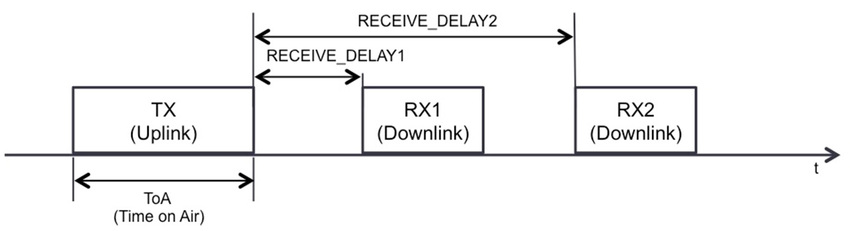
\includegraphics[width=\linewidth]{images/lorawan_class_a.png}
    \caption{LoRaWAN class A device operation.}
    \label{img: lorawan class a}
\end{figure}

\section{Real Word Use Case Scenario}
To better understand the limitations and the strengths of LoRaWAN and Bacco, we will now describe 3 real-world scenarios
in which \gls{IoT} can be integrated to achieve the benefits described in Section \ref{sec: benefits}. All of them
require to collect data on a vineyard, however, the positions and the surface areas of the vineyards are
different for the 3 cases. A brief description of each of them follows:
\begin{enumerate}
    \item A small vineyard with an area of 1 hectare \footnote{1 hectare is equivalent to $10^4~\mathrm{m^2}$} which is
        fully covered by the signal of one or more hotspots registered on a public LoRaWAN
        network. The surface of the terrain is almost flat;
    \item A small vineyard with an area of 1 hectare which is located far from any urban area and is not
        in reach from any public hotspot. The surface of the terrain is almost flat;
    \item A large vineyard with an area of 100 hectares which is located far from any urban area and is not in reach
        from any public hotspot. The vineyard is spread across multiple hills.
\end{enumerate}

\subsection{LoRaWAN Setup Using A Public Gateway}
We will now analyze an \gls{IoT} network that makes use of public infrastructures such as
\gls{TTN} or Helium. Each sender node can be easily registered on the platform and can transmit independently.\\
When trying to apply this solution to each of the described scenarios, we would observe the following behavior:
\begin{enumerate}
    \item Since the vineyard is covered by one or more public hotspots, it is possible to build the desired system.
        Depending on the distance from the hotspot, the sender nodes may be required to transmit at a high power in
        order for the signal to be detected by the hotspot. Any fault of nearby hotspots will result in an unusable
        system;
    \item Since the vineyard is not fully covered by any public LoRaWAN network, it is not possible to build the desired
        system;
    \item Since the vineyard is not fully covered by any public LoRaWAN network, it is not possible to build the desired
        system.
\end{enumerate}
\\
This is the simplest and cheapest proposed solution to implement, as no additional hardware is needed other than the
sender nodes, however, it does not satisfy the requirements for 2 out of the 3 proposed scenarios.

\subsection{LoRaWAN Setup Using An Owned Gateway}
We will now analyze an \gls{IoT} network that makes use of owned/private LoRaWAN hotspots. Each
sender node can be connected to it and can transmit independently.\\
When trying to apply this solution to each of the described scenarios, we would observe the following behavior:
\begin{enumerate}
    \item Since the vineyard is small and the underlying surface is mostly flat, the hotspot can fully cover it. The
        system satisfies the requirements;
    \item Since the vineyard is small and the underlying surface is mostly flat, the hotspot can fully cover it. The
        system satisfies the requirements;
    \item Since the vineyard is large and spread across multiple hills, it may not be possible for a single hotspot to
        cover the entirety of it because of physical barriers, so multiple hotspots would be needed to satisfy the
        requirements.
\end{enumerate}
\\
The solution satisfies the requirements for all the scenarios, however, in the $3^{rd}$ case, it is necessary to use
multiple gateways to achieve full coverage. This makes the system expensive and difficult to configure.

\subsection{Bacco Setup}
Bacco is proposed and described in this thesis as an alternative to the discussed existing solutions. It has the goal to
satisfy the requirements for the scenarios and to provide a competitive system to LoRaWAN in the field of
agriculture. The next chapters will describe its implementation in detail and compare its performance to LoRaWAN's.
